\documentclass[
  DIV=15,
  bibliography=totoc,     % Literatur im Inhaltsverzeichnis
  captions=tableheading,  % Tabellenüberschriften
  titlepage=firstiscover, % Titelseite ist Deckblatt
]{scrartcl}

% Paket float verbessern
\usepackage{scrhack}

% Warnung, falls nochmal kompiliert werden muss
\usepackage[aux]{rerunfilecheck}

% deutsche Spracheinstellungen
\usepackage{polyglossia}
\setmainlanguage{german}

% unverzichtbare Mathe-Befehle
\usepackage{amsmath}
% viele Mathe-Symbole
\usepackage{amssymb}
% Erweiterungen für amsmath
\usepackage{mathtools}

% Fonteinstellungen
\usepackage{fontspec}
% Latin Modern Fonts werden automatisch geladen

\usepackage[
  math-style=ISO,    % ┐
  bold-style=ISO,    % │
  sans-style=italic, % │ ISO-Standard folgen
  nabla=upright,     % │
  partial=upright,   % ┘
  warnings-off={           % ┐
    mathtools-colon,       % │ unnötige Warnungen ausschalten
    mathtools-overbracket, % │
  },                       % ┘
]{unicode-math}

% traditionelle Fonts für Mathematik
\setmathfont{Latin Modern Math}
\setmathfont{XITS Math}[range={scr, bfscr}]
\setmathfont{XITS Math}[range={cal, bfcal}, StylisticSet=1]

% Zahlen und Einheiten
\usepackage[
  locale=DE,                 % deutsche Einstellungen
  separate-uncertainty=true, % immer Fehler mit \pm
  per-mode=reciprocal,       % ^-1 für inverse Einheiten
  % output-decimal-marker=.,   % . statt , für Dezimalzahlen
]{siunitx}

% chemische Formeln
\usepackage[
  version=4,
  math-greek=default, % ┐ mit unicode-math zusammenarbeiten
  text-greek=default, % ┘
]{mhchem}

% richtige Anführungszeichen
\usepackage[autostyle]{csquotes}

% schöne Brüche im Text
\usepackage{xfrac}

% Standardplatzierung für Floats einstellen
\usepackage{float}
\floatplacement{figure}{htbp}
\floatplacement{table}{htbp}

% Floats innerhalb einer Section halten
\usepackage[
  section, % Floats innerhalb der Section halten
  below,   % unterhalb der Section aber auf der selben Seite ist ok
]{placeins}

% Seite drehen für breite Tabellen
\usepackage{pdflscape}

% Captions schöner machen.
\usepackage[
  labelfont=bf,        % Tabelle x: Abbildung y: ist jetzt fett
  font=small,          % Schrift etwas kleiner als Dokument
  width=0.9\textwidth, % maximale Breite einer Caption schmaler
]{caption}
% subfigure, subtable, subref
\usepackage{subcaption}

% Grafiken können eingebunden werden
\usepackage{graphicx}
% größere Variation von Dateinamen möglich
\usepackage{grffile}

% schöne Tabellen
\usepackage{booktabs}

% Verbesserungen am Schriftbild
\usepackage{microtype}

% Literaturverzeichnis
\usepackage[
  backend=biber,
]{biblatex}
% Quellendatenbank
\addbibresource{lit.bib}
\addbibresource{programme.bib}

% Hyperlinks im Dokument
\usepackage[
  unicode,        % Unicode in PDF-Attributen erlauben
  pdfusetitle,    % Titel, Autoren und Datum als PDF-Attribute
  pdfcreator={},  % ┐ PDF-Attribute säubern
  pdfproducer={}, % ┘
]{hyperref}
% erweiterte Bookmarks im PDF
\usepackage{bookmark}

% Trennung von Wörtern mit Strichen
\usepackage[shortcuts]{extdash}

\titlehead{
        
\includegraphics[height= 2cm]{./logos/FFSLogo.jpeg}
        \hfill
        
\includegraphics[height= 1cm]{./logos/tu_logo.jpg}
        }

\author{
  Pelle Ofenbach%
  \texorpdfstring{
    \\
    \href{mailto:authorA@udo.edu}{pelle.ofenbach@udo.edu}
  }{}%
  \texorpdfstring{\and}{, }
  Robert Appel%
  \texorpdfstring{
    \\
    \href{mailto:authorB@udo.edu}{robert.appel@udo.edu}
  }{}%
}
\publishers{TU Dortmund – Fakultät Physik}

%\documentclass[
  DIV=15,
  bibliography=totoc,     % Literatur im Inhaltsverzeichnis
  captions=tableheading,  % Tabellenüberschriften
  titlepage=firstiscover, % Titelseite ist Deckblatt
]{scrartcl}

% Paket float verbessern
\usepackage{scrhack}

% Warnung, falls nochmal kompiliert werden muss
\usepackage[aux]{rerunfilecheck}

% deutsche Spracheinstellungen
\usepackage{polyglossia}
\setmainlanguage{german}

% unverzichtbare Mathe-Befehle
\usepackage{amsmath}
% viele Mathe-Symbole
\usepackage{amssymb}
% Erweiterungen für amsmath
\usepackage{mathtools}

% Fonteinstellungen
\usepackage{fontspec}
% Latin Modern Fonts werden automatisch geladen

\usepackage[
  math-style=ISO,    % ┐
  bold-style=ISO,    % │
  sans-style=italic, % │ ISO-Standard folgen
  nabla=upright,     % │
  partial=upright,   % ┘
  warnings-off={           % ┐
    mathtools-colon,       % │ unnötige Warnungen ausschalten
    mathtools-overbracket, % │
  },                       % ┘
]{unicode-math}

% traditionelle Fonts für Mathematik
\setmathfont{Latin Modern Math}
\setmathfont{XITS Math}[range={scr, bfscr}]
\setmathfont{XITS Math}[range={cal, bfcal}, StylisticSet=1]

% Zahlen und Einheiten
\usepackage[
  locale=DE,                 % deutsche Einstellungen
  separate-uncertainty=true, % immer Fehler mit \pm
  per-mode=reciprocal,       % ^-1 für inverse Einheiten
  % output-decimal-marker=.,   % . statt , für Dezimalzahlen
]{siunitx}

% chemische Formeln
\usepackage[
  version=4,
  math-greek=default, % ┐ mit unicode-math zusammenarbeiten
  text-greek=default, % ┘
]{mhchem}

% richtige Anführungszeichen
\usepackage[autostyle]{csquotes}

% schöne Brüche im Text
\usepackage{xfrac}

% Standardplatzierung für Floats einstellen
\usepackage{float}
\floatplacement{figure}{htbp}
\floatplacement{table}{htbp}

% Floats innerhalb einer Section halten
\usepackage[
  section, % Floats innerhalb der Section halten
  below,   % unterhalb der Section aber auf der selben Seite ist ok
]{placeins}

% Seite drehen für breite Tabellen
\usepackage{pdflscape}

% Captions schöner machen.
\usepackage[
  labelfont=bf,        % Tabelle x: Abbildung y: ist jetzt fett
  font=small,          % Schrift etwas kleiner als Dokument
  width=0.9\textwidth, % maximale Breite einer Caption schmaler
]{caption}
% subfigure, subtable, subref
\usepackage{subcaption}

% Grafiken können eingebunden werden
\usepackage{graphicx}
% größere Variation von Dateinamen möglich
\usepackage{grffile}

% schöne Tabellen
\usepackage{booktabs}

% Verbesserungen am Schriftbild
\usepackage{microtype}

% Literaturverzeichnis
\usepackage[
  backend=biber,
]{biblatex}
% Quellendatenbank
\addbibresource{lit.bib}
\addbibresource{programme.bib}

% Hyperlinks im Dokument
\usepackage[
  unicode,        % Unicode in PDF-Attributen erlauben
  pdfusetitle,    % Titel, Autoren und Datum als PDF-Attribute
  pdfcreator={},  % ┐ PDF-Attribute säubern
  pdfproducer={}, % ┘
]{hyperref}
% erweiterte Bookmarks im PDF
\usepackage{bookmark}

% Trennung von Wörtern mit Strichen
\usepackage[shortcuts]{extdash}

\titlehead{
        
\includegraphics[height= 2cm]{./logos/FFSLogo.jpeg}
        \hfill
        
\includegraphics[height= 1cm]{./logos/tu_logo.jpg}
        }

\author{
  Pelle Ofenbach%
  \texorpdfstring{
    \\
    \href{mailto:authorA@udo.edu}{pelle.ofenbach@udo.edu}
  }{}%
  \texorpdfstring{\and}{, }
  Robert Appel%
  \texorpdfstring{
    \\
    \href{mailto:authorB@udo.edu}{robert.appel@udo.edu}
  }{}%
}
\publishers{TU Dortmund – Fakultät Physik}

\subject{ Versuch Nr. V48 }
\title{ \texorpdfstring{Dipolrelaxation in Ionenkristallen}}
\date{
  Durchführung: \printdate{ 2018-01-24 }
  \hspace{1em}
  1.Abgabe: \printdate{ 2018-02-11 }
}

\begin{document}

\maketitle
\thispagestyle{empty}
\tableofcontents
\newpage
\section{Theorie}
\label{sec:Theorie}

\subsection{Zeeman-Effekt}
Der sog. Zeeman-Effekt beschreibt die Aufspaltung der Energieniveaus von Atomen unter Einfluss eines äußeren Magnetfeldes.
Sein Ursprung liegt im magnetischen Moment $\mu_F$ der Atome, welches durch den Gesamtdrehimpuls
\begin{equation}
  \vec{\text{F}}=\vec{\text{L}}+\vec{\text{S}}+\vec{\mathbf{I}}
  \label{eqn:F}
\end{equation}
hervorgerufen wird. $\vec{\text{L}}$ bezeichnet hierbei den Bahndrehimpuls der Hüllenelektronen, $\vec{\text{S}}$ ihren Spin und $\vec{\mathbf{I}}$ den Kernspin. Diese Kopllung ist in Abb. \ref{fig:F} graphisch dargestellt.
Über die Quantenzahl $|I-J|<\text{F}<I+J$ lässt sich das Magnetische Moment nun durch

\begin{equation}
  \mu_F = \mu_B \text{g}_\text{F} \sqrt{F(F+1)}
  \label{eqn:mu_F}
\end{equation}
berechnen, wobei $\mu_B$ das Bohrsche Magneton und $\text{g}_\text{F}$  den sogenannten Landéfaktor bezeichnet.

Dieses Moment sorgt dafür, dass bei einem äußeren Magnetfeld $B$ die Energieniveaus der durch den Kernspin hervorgerufenen Hyperfeinstruktur in $2\text{F}-1$ durch eine weitere Quantenzahl $-\text{F}<\text{m}_\text{F}<\text{F}$ identifizierbare Zeeman-Niveaus aufgespalten werden. Für die Energiedifferenz zwischen diesen Niveaus gilt
\begin{equation}
  U_{Z}=\text{g}_\text{F}\mu_B B
  \label{eqn:U}
\end{equation}
Eine schematische Darstellung dieser Aufspaltung ist in Abb. \ref{fig:Zeemann} für $\mathbf{I}= \frac{2}{3}$ gegeben.
$\text{g}_\text{F}$ lässt sich mit einigen Vorüberlegungen aus den Drehimpulsquantenzahlen sowie

\begin{equation}
  \text{g}_\text{F}
  \label{eqn:gf}
\end{equation}

\newpage
\section{Durchführung}
\label{sec:Durchführung}
\subsection{Versuchsaufbau und Funktionsweise der Schaltung}
\label{sub:aufbau}
Um die Individuallebensdauern von Myonen mithilfe eines Szinzillationsdetektors zu messen, wird die Schaltung aus Abbildung \ref{fig:schaltung} verwendet.
\begin{figure}[H]
  \centering
  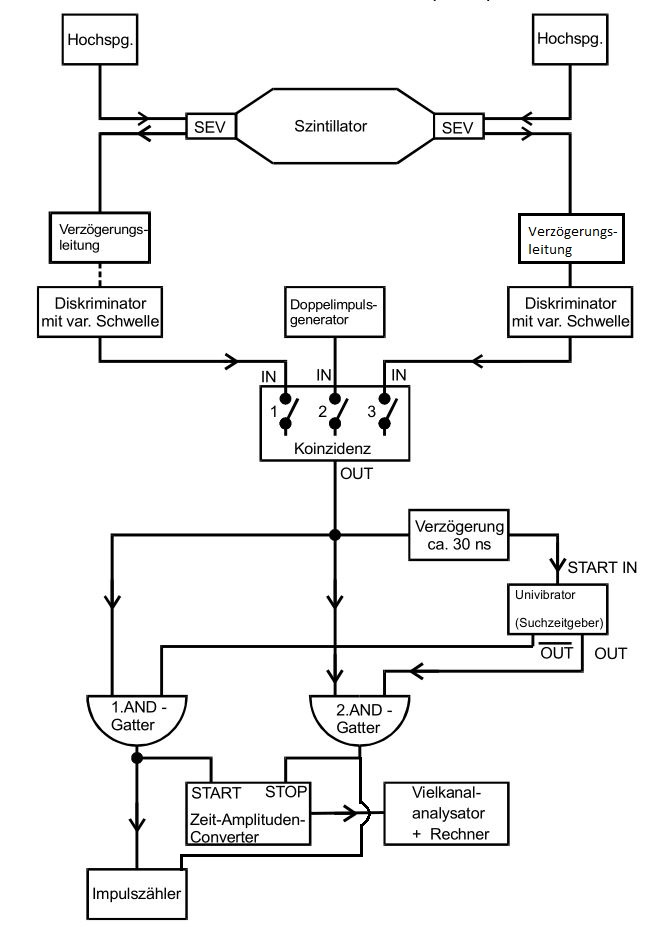
\includegraphics{./content/blockschaltbild.JPG}
  \caption{Blockschaltbild der verwendeten Schaltung nach \cite{Anleitung}}
  \label{fig:schaltung}
\end{figure}
Also Szintillationsdetetektor wird ein Edelstahlzylinder mit aufgeschweisten Kegelstümpfen verwendet, der mit einem in Toluol gelösten, organischen Szintillator gefüllt ist. Auf den Seitenflächen werden je ein an eine Hochspannung angeschlossener Sekundärelektronenvervielfacher (SEV) angeschlossen. Der SEV wird optisch an den Szintillator gekoppelt und besteht aus einer Photokathode und Dynoden zur Signalverstärkung.\\
Weiterhin werden an beide SEV eine Verzögerungsschaltung und ein Diskriminator angeschlossen. Die Verzögerungsschaltung dienen dazu die Signale der SEV, möglichst gleichzeitig in die Koinzidenzschaltung weiterzugeben. Der Diskriminator hat zwei für den weiteren Verlauf nötige Funktionen.
Ursachen für die unterschiedlichen Registrierungszeitpunkte sind zum Beispiel elektronisch unterschiedliche Eigenschaften der SEV und
\begin{itemize}
  \item[1.] Das durch z.B. thermische Elektronenemissionen in einem der SEV entstehende Rauschen wird durch Einstellen einer Signalschwelle minimiert. Die Signalschwelle ist zwischen 10 und 40 einstellbar und wird hier möglichst hoch gewählt, damit möglichst viele Myonen registriert werden können.
  \item[2.] Das einlaufende Signal wird in ein H/L-Signal der NIM-Logik übersetzt, damit die anschließend verwendeten Logikbausteine das Signal verarbeiten können.
\end{itemize}
Das Übersetzen der Signale in NIM-Logik ist hierbei die Hauptaufgabe des Diskriminators, da die Selektion der Signale durch effizienter durch die im Folgenden erklärte Koinzidenzschaltung vorgenommen wird. Die aus den Diskriminatoren auslaufenden Signale werden nun auf eine Koinzidenzschaltung gegeben. Diese dient dazu diejenigen Signale auszusortieren, welche durch durch thermische Emissionen in einem der SEV entstehen. Wird ein Myon nah an einem der beiden SEV gemessen, ist es möglich, dass die nachfolgende Schaltung die Messung irrtümlich als fehlgeschlagen interpretiert, da die Lichtimpulse zu unterschiedlichen Zeiten von den SEV registriert werden. Dieses Problem wird ebenfalls durch die Koinzidenzschaltung minimiert.\\
Aus der Koinzidenschaltung wird das Signal nun dreigeteilt und auf zwei AND-Gatter sowie durch eine weitere Verzögerung in eine monostabile Kippstufe geleitet. Die Kippstufe wird ebenfalls an die beiden AND-Gatter angeschlossen. Wird nun ein Myon detektiert, liegt am Eingang des ersten AND-Gatters ein H an. Da die Kippstufe noch nicht gekippt ist gibt das Gatter ein H Signal weiter, bis nach $\SI{30}{\nano\second}$ die Stufe kippt und das H Signal am $\bar{\symup{\bar{OUT}}}$ anliegt. Falls im Detektor nun ein zweiter Puls aufgenommen wird, wird dieser durch das zweite AND-Gatter als H Signal weitergeleitet. Das erste Gatter registriert also den Eintritt und das zweite den Zerfall des Myons. Die Signale der Gatter werden nun von je einem Impulszähler registriert und in einen Zeit-Amplitude-Konverter (TAC) geleitet. Dieser wandelt die zwischen den Pulsen vergehende Zeit in ein Signal mit Höhe proportional zur vergangen Zeit um. Diese Signale werden dann mithilfe eines Analog-Digital Konverters in einem Vielkanalanalysator geleteitet. Die am TAC entstehenden Signale sind also repräsentativ für die Individuallebensdauern der Myonen.\\
\subsection{Kalibrierung und Messverfahren}
\label{sub:kalimes}
Bevor die eigentliche Messung durchgeführt werden kann wird die Schaltung der Reihe nach aufgebaut und das Signal mithilfe eines Oszilloskops visualisiert um die idealen Kenngrößen einzustellen.
Zu erst werden die Verzögerer richtig eingestellt und die Breite der Spannungspulse wird vermessen.
Dann werden die Diskriminatoren angeschlossen und die Diskriminatorschwelle so eingestellt, dass beide Messkanäle ungefähr gleiche Zählraten liefern.
Auch hier wird die Breite der nun rechteckigen Pulse ausgelesen.\\
Als nächstes wird die Koinzidenzschaltung justiert. Dafür wird die Verzögerungszeit systematisch variiert und die unterschiedlichen Zählraten werden aufgenommen.
Das Maximum der entstehenden Kurve wird als ideale Verzögerungszeit eingestellt. Des weiteren wird die Zählrate vor und nach der Koinzidenzschaltung verglichen um sich von der Wirksamkeit der Schaltung
zu überzeugen.\\
Anschließed werden die Kippstufe, die AND-Gatter und der TAC angeschlossen. Am Ausgang des TAC kann nun die Suchzeit gemessen werden, in der die Stufe sich im gekippten Zustand befindet.
Die Suchzeit sollte dabei nur wenig größer sein als die Messzeit des TAC. Die Suchzeit beträgt $T_s = $. Mithilfe eines ebenfalls an die Koinzidenzschaltung angeschlossenen Doppelimpulsgenerators wird die Funktionsweise der Schaltung zur Registrierung des Stoppimpulses getestet. Dies ist notwendig, da im späteren Experiment nur wenige der eintretenden Myonen auch im Detektor zerfallen. Am TAC wird nun außerdem überprüft ob die ausgehenden Signale proportional zum am Doppelimpulsgenerator eingestellten Impulsabstand sind.\\
Zuletzt wird die Kalibration des Vielkanalysators vorgenommen. Dafür wird überprüft welcher Kanal welcher Messzeit entspricht.\\
\\
Nun kann mit der eigentlichen Messung der Individuallebensdauern begonnen werden. Dafür werden Zählwerk und Vielkanalanalysator zeitgleich gestartet. Die Messung läuft über ca. 25 Stunden und wird wiederum durch gleichzeitiges Stoppen der Zählwerks und des Vielkanalanalysators beendet. Die Ergebnisse des Vielkanalanalysators, sowie die Anzahl der detektierten Start- und Stoppimpulse werden aufgezeichnet und die exakte Messzeit werden aufgezeichnet.\\

\newpage
\section{Auswertung}
\label{sec:Auswertung}
\subsection{Kalibrierung}
\begin{figure}
  \includegraphics{./plots/plot.pdf}
  \caption{Ereignisraten nach Hinzuschalten der Koinzidenzschaltung in Abhängigkeit der eingestellten relativen Verzögerung der Signale zueinander.}
  \label{fig:koinzidenz}
\end{figure}
\begin{table}
  \caption{Länge der vom linken, bzw. rechten, Detektor ausgegebenen Impulse ohne Hinzuschalten eines Diskriminators}
  \label{tab:oD}
  \centering
  \begin{tabular}{|S|S|}
    \toprule
    $t_{links}/\si{\nano \second}$ & $t_{rechts}/\si{\nano \second}$\\
    \midrule
    6,6 & 10,2 \\
    8,6 & 7,8 \\
    8,2 & 10,4 \\
    10,0 & 7,6 \\
    14,0 & 9,4 \\
    9,0 & 11,8 \\
    10,6 & 8,4 \\
    8,6 & 12,0 \\
    10,4 & 7,6 \\
    11,0 & 10,0 \\
    \toprule
  \end{tabular}
\end{table}

Nach Hinzuschalten der Diskriminatoren beträgt $t_{links}= \SI{19,6}{\nano\second}$ und $t_{rechts} = \SI{19,0}{\nano \second}$. Die Diskriminatoren sind hierbei so aufeinander abgestimmt, dass sich ihre Ereignisfrequenzen nur um $\Delta_f = \SI{0,05}{\per \second}$ unterscheiden. Ihre Ereignisfrequenzen liegen bei $f_{links} = \SI{38.27}{\per \second}$, bzw. $f_{rechts}= \SI{38,22}{\per \second}$.

\begin{table}
  \caption{Nach der Koinzidenzschaltung registrierte Ereignisse in Abhängigkeit der relativen Verzögerung der Signale zueinander.}
  \label{tab:koinzidenz}
  \centering
  \begin{tabular}{|S|S|S|}
    \toprule
    $t_{VZ}/\si{\nano\second}$ & $\text{Ereignisse/}\si{\per\second}$ & $\text{Messzeit}/\si{\second}$ \\
    \midrule
    0.0 & 421 \pm 21 & 20.22 \\
    16.0 & 422 \pm 21& 21.39  \\
    20.0 & 285 \pm 17& 20.20 \\
    22.0 & 174 \pm 13 & 20.24 \\
    23.0 & 116 \pm 11& 19.96 \\
    23.5 & 85 \pm 9& 20.06 \\
    -8.0 & 470 \pm 22& 20.36 \\
    -40.0 & 14 \pm 4 & 20.45 \\
    8.0 & 441 \pm 21& 19.98 \\
    12.0 & 451 \pm 21& 20.05 \\
    -24.0 & 10 \pm 3 & 20.42 \\
    -28.0 & 10 \pm 3& 20.42 \\
    -20.0 & 169\pm13 & 20.03 \\
    -22.0 & 63 \pm 8& 20.16 \\
    -18.0 & 282 \pm 17&20.30 \\
    -17.0 & 301 \pm17& 20.15 \\
    -19.0 & 211 \pm 15& 20.40 \\
    -10.0 & 449 \pm 21& 20.23 \\
    1.0 & 479 \pm 22& 20.59 \\
    -12.0 & 426 \pm21& 20.10 \\
    0.0 & 463 \pm22& 20.05 \\
    \bottomrule
  \end{tabular}
\end{table}

Für die relative Verzögerungszeit $t_{VZ}= \SI{0.0}{\nano\second}$ wurden zwei Messwerte aufgenommen, da sie sich sehr nah am gemessenen Maximum von $t_{VZ}= \SI{1.0}{\nano\second}$ befindet und die erste Messung einen recht stark abweichenden Wert zeigt, obwohl ein ausgeprägtes Platau erwartet wird. Die in Tab. \ref{tab:koinzidenz} gelisteten Messwerte sind in Abb. \ref{fig:koinzidenz} graphisch dargestellt. Die Plateaurate $f_p$ wurde über die markierten Werte mittels NumPy \cite{numpy} gemittelt und ergibt sich zu $f_p = \SI{22.16}{\per\second}$. Durch Anlegen einer Geraden der Form $f = ax+b$ an die ebenfalls markierten Werte der Flanken der Verteilung durch lineare Regression mittels Python \cite{matploitlib} kann durch die Schnittpunkte $f_{h,l}$ und ${f_h,r}$ dieser Geraden mit der Hälfte des Plateaus $\Delta t_k = \SI{40}{\nano\second}-\left(f_{h,r}-f_{h,l}\right) = \SI{0.57\pm 0.30}{\nano \second}$ berechnen.

Die Parameter der Ausgleichsgeraden lauten hierbei:
\begin{align*}
  &a_{links}&= \SI{2.06\pm 0.21}{\per\nano\second\squared}, &a_{rechts} &= \SI{-2.44\pm 0.16}{\per\nano\second\squared}\\
  &b_{links} &= \SI{54\pm4}{\per \second}, &b_{rechts} &= \SI{57.0\pm 3.1}{\per\second}
\end{align*}

\begin{table}
  \caption{Unbearbeitete Messwerte zur Kalibrierung des Vielkanalanalysators}
  \centering
  \label{tab:kanal}
    \begin{tabular}{|S|S|S|}
      \hline
      $t/\si{\micro\second}$ & $\text{Kanal}$ & $\text{Counts}$ \\ \hline

      1 & 22 & 5055 \\
      1 & 23 & 999 \\ \hline
      2 & 44 & 196 \\
      2 & 45 & 4075 \\ \hline
      3 & 67 & 3815 \\ \hline
      4 & 89 & 4863 \\ \hline
      5 & 111 & 5904 \\ \hline
      6 & 133 & 5612 \\ \hline
      7 & 155 & 899 \\ \hline
      8 & 177 & 6509 \\ \hline
      9 & 199 & 7437 \\\hline
    \end{tabular}
\end{table}

\begin{table}
  \caption{Kanäle mit vom Doppelimpulsgenerator vorgegebenen Zeitintervallen sowie ihr Abstände}
  \label{tab:Kalibrierung}
  \centering
  \sisetup{round-mode = places , round-precision = 2,scientific-notation=fixed, fixed-exponent = 0}
  \begin{tabular}{|S|S|}
    \toprule
    $\text{Kanal}$ & $\text{Abstand}$ \\
    \midrule
    22.16501487   & 22.16501487 \\
    44.95410911   & 22.78909424 \\
    67.           & 22.04589089 \\
    89.           & 22 \\
    111.          & 22 \\
    133.          & 22 \\
    155.          & 22 \\
    177.          & 22 \\
    199.          & 22 \\
    \bottomrule
  \end{tabular}
\end{table}

Aus den in Tab. \ref{tab:Kalibrierung} aufgeführten Werten (gemittelt aus Tab. \ref{tab:kanal} nach \eqref{kanalmittel}) ergibt sich eine Umrechnung von $(22.11 \pm 0.08) \, \frac{\text{Kanäle}}{\si{\micro\second}}$.

\subsection{Messung der Individuallebensdauern kosmischer Myonen}

\begin{figure}
  \centering
  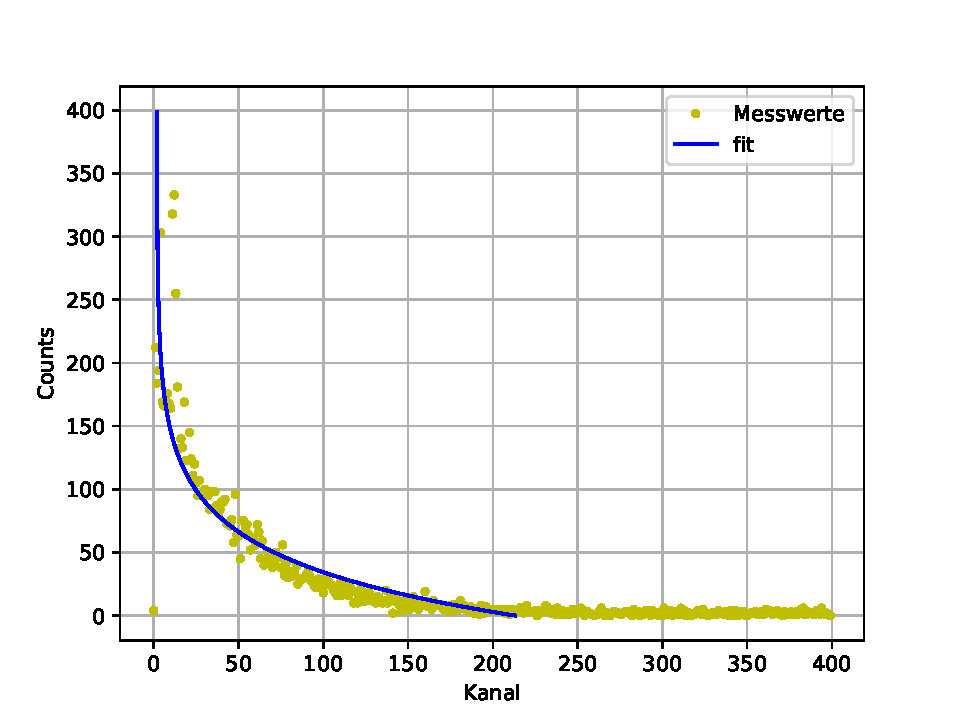
\includegraphics{./plots/lebensdauer.pdf}
  \caption{Gemessene Individuallebensdauern der detektierten Myonen}
  \label{fig:tau}
\end{figure}


Ein mittels $matplotlib$ \cite{matplotlib} über die Methode der kleinsten Quadrate durchgeführter ungewichteter Fit der Werte der Individuallebensdauern (dargestellt in Abb. \ref{fig:tau}) an eine Exponentialfunktion der Form $f(t) = A \exp\left(-\tau t\right)+U$ liefert folgende Werte:
\begin{align*}
  \tau &= \SI{2.03 \pm 0.09}{\micro\second} \\
  U &= 1.9 \pm 1.2 \\
  A &= 211 \pm 5
\end{align*}

Hierbei bezeichnet $U$ einen konstanten Untergrund aus zufällig, gleichverteilt auftretenden Ereignissen und $A$ als Ordinatenabschnitt.
Hierbei wurden die leeren ersten beiden Kanäle, sowie die ebenfalls leeren Kanäle 401 bis 511, bei der Auswertung der Daten vernachlässigt. Die ersten beiden Kanäle decken eine Zeit von ca. $t_{tot} = \SI{0.09}{\micro \second}$ ab.
Hierbei fällt auf, dass die Zahl der MCA gemessenen Ereignisse mit $C_{MCA}=10311.0$ geringer ist als die 10868 seperat gemessenen Stop Signale.


Mit $2096502$ detektierten Startimpulsen werden bei einer Messzeit von $\SI{96454}{\second}$ wird nach Gl. \eqref{eqn:barN} eine durchschnittliches Rauschen von $\SI{21.74}{\per \second}$ erwartet. Der Untergrund pro Kanal wird somit gemäß \eqref{eqn:Untergrund} mit $U = 1.7793 \pm 0.0025$ erwartet.


% \begin{figure}
%   \centering
%   \includegraphics{plot.pdf}
%   \caption{Plot.}
%   \label{fig:plot}
% \end{figure}



% \begin{table}
%    % Notation :  {% nicht entfernen ist sehr wichtig sonst Fehler !!
% \parbox{0.48\textwidth}{% %Ermöglicht zwei Tabellen neben einander
%   \centering
%   \sisetup{round-mode = places , round-precision = 0,scientific-notation=fixed, fixed-exponent = 0}
%          %rundet Werte aus Stelle, Stelle = ,  macht einen bestimmten festen exponenten
%   \resizebox{\textwidth}{!}{%  % skaliert zu große Tabellen
%   \begin{tabular}{S@{${}\pm{}$} S} % fügt plus minus Fehler Schreibweise hinzu
%     \toprule
%      $\text{e}_b / \si{\milli\meter}$ &
%      $\text{d}_b /\si{\milli\meter} $ & $\text{f}_b / \si{\milli\meter} $\\
%     \midrule
%     \bottomrule
%   \end{tabular}
%   % }
%   \caption{Tabellenunterschrift}
%   \label{tab:tab}
% }
% % \end{table}
% % \begin{table}
% \parbox{0.48\textwidth}{%
%   \centering
%   \sisetup{round-mode = places , round-precision = 0,scientific-notation=fixed, fixed-exponent = 0}
%   % \resizebox{\textwidth}{!}{%
%   \begin{tabular}{S@{${}\pm{}$} S}
%     \toprule
%      $\text{e}_b / \si{\milli\meter}$ &
%      $\text{d}_b /\si{\milli\meter} $ & $\text{f}_b / \si{\milli\meter} $\\
%     \midrule
%     \bottomrule
%   \end{tabular}
%   % }
%   \caption{Tabellenunterschrift}
%   \label{tab:tab}
% }
% \end{table}

\section{Diskussion}
\label{sec:Diskussion}
\subsection{Relativer Fehler}
Alle relativen Fehler wurden nach der Formel
\begin{equation*}
  \tilde{x} = \frac{ \lvert x_{lit} - x_{mess} \rvert}{\lvert x_{lit} \rvert}
  \cdot 100 \%
\end{equation*}
berechnet, dabei bezeichnet $x_{lit}$ den Literaturwert der Messgröße $x_{mess}$.

\section{Tabellen}
\label{sec:Tabellen}
\begin{table}[H]
  \centering
  \caption{Umgerechnete Messwerte der 1.Messung $(b_\text{heiz} = \SI{1.5}{\kelvin\per\minute})$}
  \label{tab:1}
    \begin{tabular}{S S S S S S}
    \toprule
    $\text{i(T)} \: / \: \num{10e-11} \, \si{\ampere} $ & $ T \: / \: \si{\kelvin}$
    & $ t \: / \: \si{\second}$ &
    $\text{i(T)} \: / \: \num{10e-11} \, \si{\ampere} $ & $ T \: / \: \si{\kelvin}$
    & $ t \: / \: \si{\second}$\\
    \midrule
    0.000 & 211.55 & 0 & 0.390 & 275.15 & 2520 \\
    0.000 & 213.95 & 60 & 0.410 & 276.75 & 2580 \\
    0.012 & 215.65 & 120 & 0.420 & 278.25 & 2640 \\
    0.024 & 217.65 & 180 & 0.440 & 279.55 & 2700 \\
    0.042 & 219.45 & 240 & 0.460 & 280.95 & 2760 \\
    0.096 & 220.85 & 300 & 0.480 & 282.35 & 2820 \\
    0.102 & 222.35 & 360 & 0.500 & 283.65 & 2880 \\
    0.105 & 223.75 & 420 & 0.520 & 285.05 & 2940 \\
    0.108 & 225.45 & 480 & 0.550 & 286.55 & 3000 \\
    0.108 & 227.25 & 540 & 0.570 & 288.05 & 3060 \\
    0.117 & 228.75 & 600 & 0.590 & 289.45 & 3120 \\
    0.123 & 229.85 & 660 & 0.610 & 290.85 & 3180 \\
    0.129 & 231.35 & 720 & 0.620 & 292.15 & 3240 \\
    0.138 & 232.95 & 780 & 0.640 & 293.65 & 3300 \\
    0.156 & 234.75 & 840 & 0.660 & 295.15 & 3360 \\
    0.180 & 236.65 & 900 & 0.680 & 296.65 & 3420 \\
    0.207 & 238.25 & 960 & 0.690 & 297.95 & 3480 \\
    0.234 & 239.45 & 1020 & 0.710 & 299.45 & 3540 \\
    0.270 & 240.85 & 1080 & 0.740 & 300.95 & 3600 \\
    0.300 & 242.15 & 1140 & 0.780 & 302.45 & 3660 \\
    0.360 & 243.45 & 1200 & 0.800 & 303.95 & 3720 \\
    0.440 & 244.95 & 1260 & 0.870 & 305.35 & 3780 \\
    0.510 & 246.65 & 1320 & 0.920 & 306.85 & 3840 \\
    0.620 & 248.05 & 1380 & 0.990 & 308.25 & 3900 \\
    0.740 & 249.55 & 1440 & 1.050 & 309.85 & 3960 \\
    0.870 & 251.05 & 1500 & 1.110 & 311.35 & 4020 \\
    1.000 & 252.55 & 1560 & 1.200 & 312.95 & 4080 \\
    1.170 & 254.05 & 1620 & 1.260 & 314.55 & 4140 \\
    1.260 & 255.55 & 1680 & 1.350 & 316.15 & 4200 \\
    1.350 & 256.95 & 1740 & 1.380 & 317.75 & 4260 \\
    1.410 & 258.35 & 1800 & 1.380 & 319.25 & 4320 \\
    1.410 & 259.75 & 1860 & 1.380 & 320.75 & 4380 \\
    1.350 & 261.15 & 1920 & 1.320 & 322.25 & 4440 \\
    1.260 & 262.75 & 1980 & 1.260 & 323.75 & 4500 \\
    1.080 & 264.25 & 2040 & 1.200 & 325.35 & 4560 \\
    0.930 & 265.65 & 2100 & 1.110 & 326.65 & 4620 \\
    0.750 & 267.05 & 2160 & 1.020 & 327.95 & 4680 \\
    0.600 & 268.45 & 2220 & 0.930 & 329.95 & 4740 \\
    0.500 & 269.95 & 2280 & 0.870 & 331.15 & 4800 \\
    0.430 & 271.35 & 2340 & 0.760 & 332.75 & 4860 \\
    0.400 & 272.65 & 2400 & 0.740 & 333.15 & 4875 \\
    0.390 & 273.95 & 2460 &       &        &      \\
    \bottomrule
  \end{tabular}
\end{table}

\begin{table}[H]
  \centering
  \caption{Umgerechnete Messwerte der 2.Messung $(b_\text{heiz} =
  \SI{3.0}{\kelvin\per\minute})$}
  \label{tab:2}
    \begin{tabular}{S S S}
    \toprule
    $ \text{i(T)}  \: / \: 10^{-11} \, \si{\ampere} $ & $ T\: / \: \si{\kelvin} $
    & $ t \: / \: \si{\second} $ \\
    \midrule
    0.000 & 213.25 & 0 \\
    0.114 & 214.85 & 60 \\
    0.114 & 216.75 & 12 \\
    0.117 & 219.25 & 180 \\
    0.126 & 222.25 & 240 \\
    0.135 & 225.25 & 300 \\
    0.147 & 228.25 & 360 \\
    0.165 & 231.35 & 420 \\
    0.189 & 234.45 & 480 \\
    0.225 & 237.45 & 540 \\
    0.290 & 240.55 & 600 \\
    0.360 & 243.35 & 660 \\
    0.510 & 246.15 & 720 \\
    0.700 & 248.95 & 780 \\
    0.980 & 251.65 & 840 \\
    1.380 & 254.55 & 900 \\
    1.920 & 257.65 & 960 \\
    2.430 & 260.75 & 1020 \\
    2.760 & 263.75 & 1080 \\
    2.640 & 266.95 & 1140 \\
    2.130 & 269.85 & 1200 \\
    1.440 & 272.65 & 1260 \\
    0.900 & 275.25 & 1320 \\
    0.780 & 277.95 & 1380 \\
    0.750 & 280.65 & 1440 \\
    0.760 & 283.45 & 1500 \\
    0.820 & 286.35 & 1560 \\
    0.910 & 289.25 & 1620 \\
    0.950 & 292.05 & 1680 \\
    1.020 & 294.75 & 1740 \\
    1.050 & 297.65 & 1800 \\
    1.080 & 300.55 & 1860 \\
    1.110 & 303.55 & 1920 \\
    1.200 & 306.55 & 1980 \\
    1.380 & 309.65 & 2040 \\
    1.590 & 312.55 & 2100 \\
    1.740 & 315.45 & 2160 \\
    1.920 & 318.35 & 2220 \\
    2.040 & 321.15 & 2280 \\
    2.040 & 323.95 & 2340 \\
    1.860 & 326.85 & 2400 \\
    1.620 & 329.65 & 2460 \\
    \bottomrule
  \end{tabular}
\end{table}

\begin{table}[H]
  \centering
  \caption{Werte des Integrals von $i(T)$ der 1.Messung $(b_\text{heiz} =
  \SI{1.5}{\kelvin\per\minute})$}
  \label{tab:3}
    \begin{tabular}{S S S S}
    \toprule
    $ T \: / \: \si{\kelvin} $ & $ \text{Integral von  i(T)} \: / \:
    \num{10e-11} \, \si{\ampere}$ & $ \text{Integral von } \Delta \text{i(T)} \: / \:
    \num{10e-11} \, \si{\ampere}$ &
    $ \text{i(T)}  \: / \:  10^{-11} \, \si{\ampere} $ \\
    \midrule
    269.950 & 0.071 & 0.079 & 0.500 \\
    268.450 & 0.289 & 0.163 & 0.600 \\
    267.050 & 0.681 & 0.242 & 0.750 \\
    265.650 & 1.318 & 0.321 & 0.930 \\
    264.250 & 2.199 & 0.399 & 1.080 \\
    262.750 & 3.406 & 0.484 & 1.260 \\
    261.150 & 4.926 & 0.574 & 1.350 \\
    259.750 & 6.376 & 0.653 & 1.410 \\
    258.350 & 7.881 & 0.731 & 1.410 \\
    256.950 & 9.357 & 0.810 & 1.350 \\
    255.550 & 10.742 & 0.889 & 1.260 \\
    254.050 & 12.106 & 0.973 & 1.170 \\
    252.550 & 13.290 & 1.058 & 1.000 \\
    251.050 & 14.264 & 1.142 & 0.870 \\
    249.550 & 15.059 & 1.226 & 0.740 \\
    248.050 & 15.682 & 1.311 & 0.620 \\
    246.650 & 16.117 & 1.389 & 0.510 \\
    244.950 & 16.509 & 1.485 & 0.440 \\
    243.450 & 16.760 & 1.569 & 0.360 \\
    242.150 & 16.898 & 1.643 & 0.300 \\
    240.850 & 16.989 & 1.716 & 0.270 \\
    239.450 & 17.055 & 1.794 & 0.234 \\
    238.250 & 17.084 & 1.862 & 0.207 \\
    236.650 & 17.094 & 1.952 & 0.180 \\
    234.750 & 17.081 & 2.059 & 0.156 \\
    232.950 & 17.054 & 2.160 & 0.138 \\
    231.350 & 17.027 & 2.250 & 0.129 \\
    229.850 & 17.006 & 2.334 & 0.123 \\
    228.750 & 16.994 & 2.396 & 0.117 \\
    227.250 & 16.980 & 2.481 & 0.108 \\
    225.450 & 16.975 & 2.582 & 0.108 \\
    223.750 & 16.988 & 2.678 & 0.105 \\
    222.350 & 17.010 & 2.756 & 0.102 \\
    220.850 & 17.041 & 2.841 & 0.096 \\
    219.450 & 17.042 & 2.919 & 0.042 \\
    217.650 & 16.999 & 3.021 & 0.024 \\
    215.650 & 16.946 & 3.133 & 0.012 \\
    \bottomrule
  \end{tabular}
\end{table}

\begin{table}[H]
  \centering
  \caption{Werte des Integrals von $i(T)$ der 1.Messung $(b_\text{heiz} =
  \SI{3.0}{\kelvin\per\minute})$}
  \label{tab:4}
    \begin{tabular}{S S S S}
    \toprule
    $ T\: / \: \si{\kelvin} $ & $ \text{Integral von  i(T)} \: / \:
    \num{10e-11} \, \si{\ampere}$ & $ \text{Integral von } \Delta \text{i(T)} \: / \:
    \num{10e-11} \, \si{\ampere}$ &
    $ \text{i(T)}  \: / \:  \num{10e-11} \, \si{\ampere} $ \\
    \midrule
    275.250 & 0.317 & 0.283 & 0.900 \\
    272.650 & 1.561 & 0.555 & 1.440 \\
    269.850 & 4.709 & 0.849 & 2.130 \\
    266.950 & 9.806 & 1.153 & 2.640 \\
    263.750 & 16.552 & 1.488 & 2.760 \\
    260.750 & 22.669 & 1.803 & 2.430 \\
    257.650 & 27.797 & 2.127 & 1.920 \\
    254.550 & 31.409 & 2.452 & 1.380 \\
    251.650 & 33.526 & 2.756 & 0.980 \\
    248.950 & 34.667 & 3.039 & 0.700 \\
    246.150 & 35.281 & 3.333 & 0.510 \\
    243.350 & 35.511 & 3.626 & 0.360 \\
    240.550 & 35.523 & 3.920 & 0.290 \\
    237.450 & 35.433 & 4.244 & 0.225 \\
    234.450 & 35.301 & 4.559 & 0.189 \\
    231.350 & 35.181 & 4.884 & 0.165 \\
    228.250 & 35.107 & 5.209 & 0.147 \\
    225.250 & 35.097 & 5.523 & 0.135 \\
    222.250 & 35.160 & 5.837 & 0.126 \\
    \bottomrule
  \end{tabular}
\end{table}

\begin{table}[H]
  \centering
  \caption{Werte für die Aktivierungsenergiebestimmung der 1.Messung
  $(b_\text{heiz} =
  \SI{1.5}{\kelvin\per\minute})$}
  \label{tab:5}
    \begin{tabular}{S S S S}
    \toprule
    $ \text{ln(j)} $ & $ T \: / \:\si{\kelvin}$
    & $ \text{ln(j)} $ & $ T \: / \:\si{\kelvin}$ \\
    \midrule
    -16.747 & 215.65 & -13.265 & 275.15 \\
    -16.054 & 217.65 & -13.215 & 276.75 \\
    -15.494 & 219.45 & -13.191 & 278.25 \\
    -14.667 & 220.85 & -13.145 & 279.55 \\
    -14.607 & 222.35 & -13.100 & 280.95 \\
    -14.578 & 223.75 & -13.058 & 282.35 \\
    -14.549 & 225.45 & -13.017 & 283.65 \\
    -14.549 & 227.25 & -12.978 & 285.05 \\
    -14.469 & 228.75 & -12.922 & 286.55 \\
    -14.419 & 229.85 & -12.886 & 288.05 \\
    -14.372 & 231.35 & -12.851 & 289.45 \\
    -14.304 & 232.95 & -12.818 & 290.85 \\
    -14.182 & 234.75 & -12.802 & 292.15 \\
    -14.039 & 236.65 & -12.770 & 293.65 \\
    -13.899 & 238.25 & -12.739 & 295.15 \\
    -13.776 & 239.45 & -12.710 & 296.65 \\
    -13.633 & 240.85 & -12.695 & 297.95 \\
    -13.528 & 242.15 & -12.666 & 299.45 \\
    -13.346 & 243.45 & -12.625 & 300.95 \\
    -13.145 & 244.95 & -12.572 & 302.45 \\
    -12.997 & 246.65 & -12.547 & 303.95 \\
    -12.802 & 248.05 & -12.463 & 305.35 \\
    -12.625 & 249.55 & -12.407 & 306.85 \\
    -12.463 & 251.05 & -12.334 & 308.25 \\
    -12.324 & 252.55 & -12.275 & 309.85 \\
    -12.167 & 254.05 & -12.219 & 311.35 \\
    -12.093 & 255.55 & -12.142 & 312.95 \\
    -12.024 & 256.95 & -12.093 & 314.55 \\
    -11.980 & 258.35 & -12.024 & 316.15 \\
    -11.980 & 259.75 & -12.002 & 317.75 \\
    -12.024 & 261.15 & -12.002 & 319.25 \\
    -12.093 & 262.75 & -12.002 & 320.75 \\
    -12.247 & 264.25 & -12.046 & 322.25 \\
    -12.396 & 265.65 & -12.093 & 323.75 \\
    -12.612 & 267.05 & -12.142 & 325.35 \\
    -12.835 & 268.45 & -12.219 & 326.65 \\
    -13.017 & 269.95 & -12.304 & 327.95 \\
    -13.168 & 271.35 & -12.396 & 329.95 \\
    -13.240 & 272.65 & -12.463 & 331.15 \\
    -13.265 & 273.95 & -12.598 & 332.75 \\
    \bottomrule
  \end{tabular}
\end{table}

\begin{table}[H]
  \centering
  \caption{Werte für die Aktivierungsenergiebestimmung der 1.Messung
  $(b_\text{heiz} =
  \SI{3.0}{\kelvin\per\minute})$}
  \label{tab:6}
    \begin{tabular}{S S S S}
    \toprule
    $ \text{ln(j)} $ & $ T \: / \:\si{\kelvin}$
    & $ \text{ln(j)} $ & $ T \: / \:\si{\kelvin}$ \\
    \midrule
    -14.495 & 214.85 & -11.959 & 272.65 \\
    -14.495 & 216.75 & -12.429 & 275.25 \\
    -14.469 & 219.25 & -12.572 & 277.95 \\
    -14.395 & 222.25 & -12.612 & 280.65 \\
    -14.326 & 225.25 & -12.598 & 283.45 \\
    -14.241 & 228.25 & -12.522 & 286.35 \\
    -14.126 & 231.35 & -12.418 & 289.25 \\
    -13.990 & 234.45 & -12.375 & 292.05 \\
    -13.816 & 237.45 & -12.304 & 294.75 \\
    -13.562 & 240.55 & -12.275 & 297.65 \\
    -13.346 & 243.35 & -12.247 & 300.55 \\
    -12.997 & 246.15 & -12.219 & 303.55 \\
    -12.681 & 248.95 & -12.142 & 306.55 \\
    -12.344 & 251.65 & -12.002 & 309.65 \\
    -12.002 & 254.55 & -11.860 & 312.55 \\
    -11.672 & 257.65 & -11.770 & 315.45 \\
    -11.436 & 260.75 & -11.672 & 318.35 \\
    -11.309 & 263.75 & -11.611 & 321.15 \\
    -11.353 & 266.95 & -11.611 & 323.95 \\
    -11.568 & 269.85 & -11.703 & 326.85 \\
    \bottomrule
  \end{tabular}
\end{table}
\section{Messwerte}

\begin{figure}
  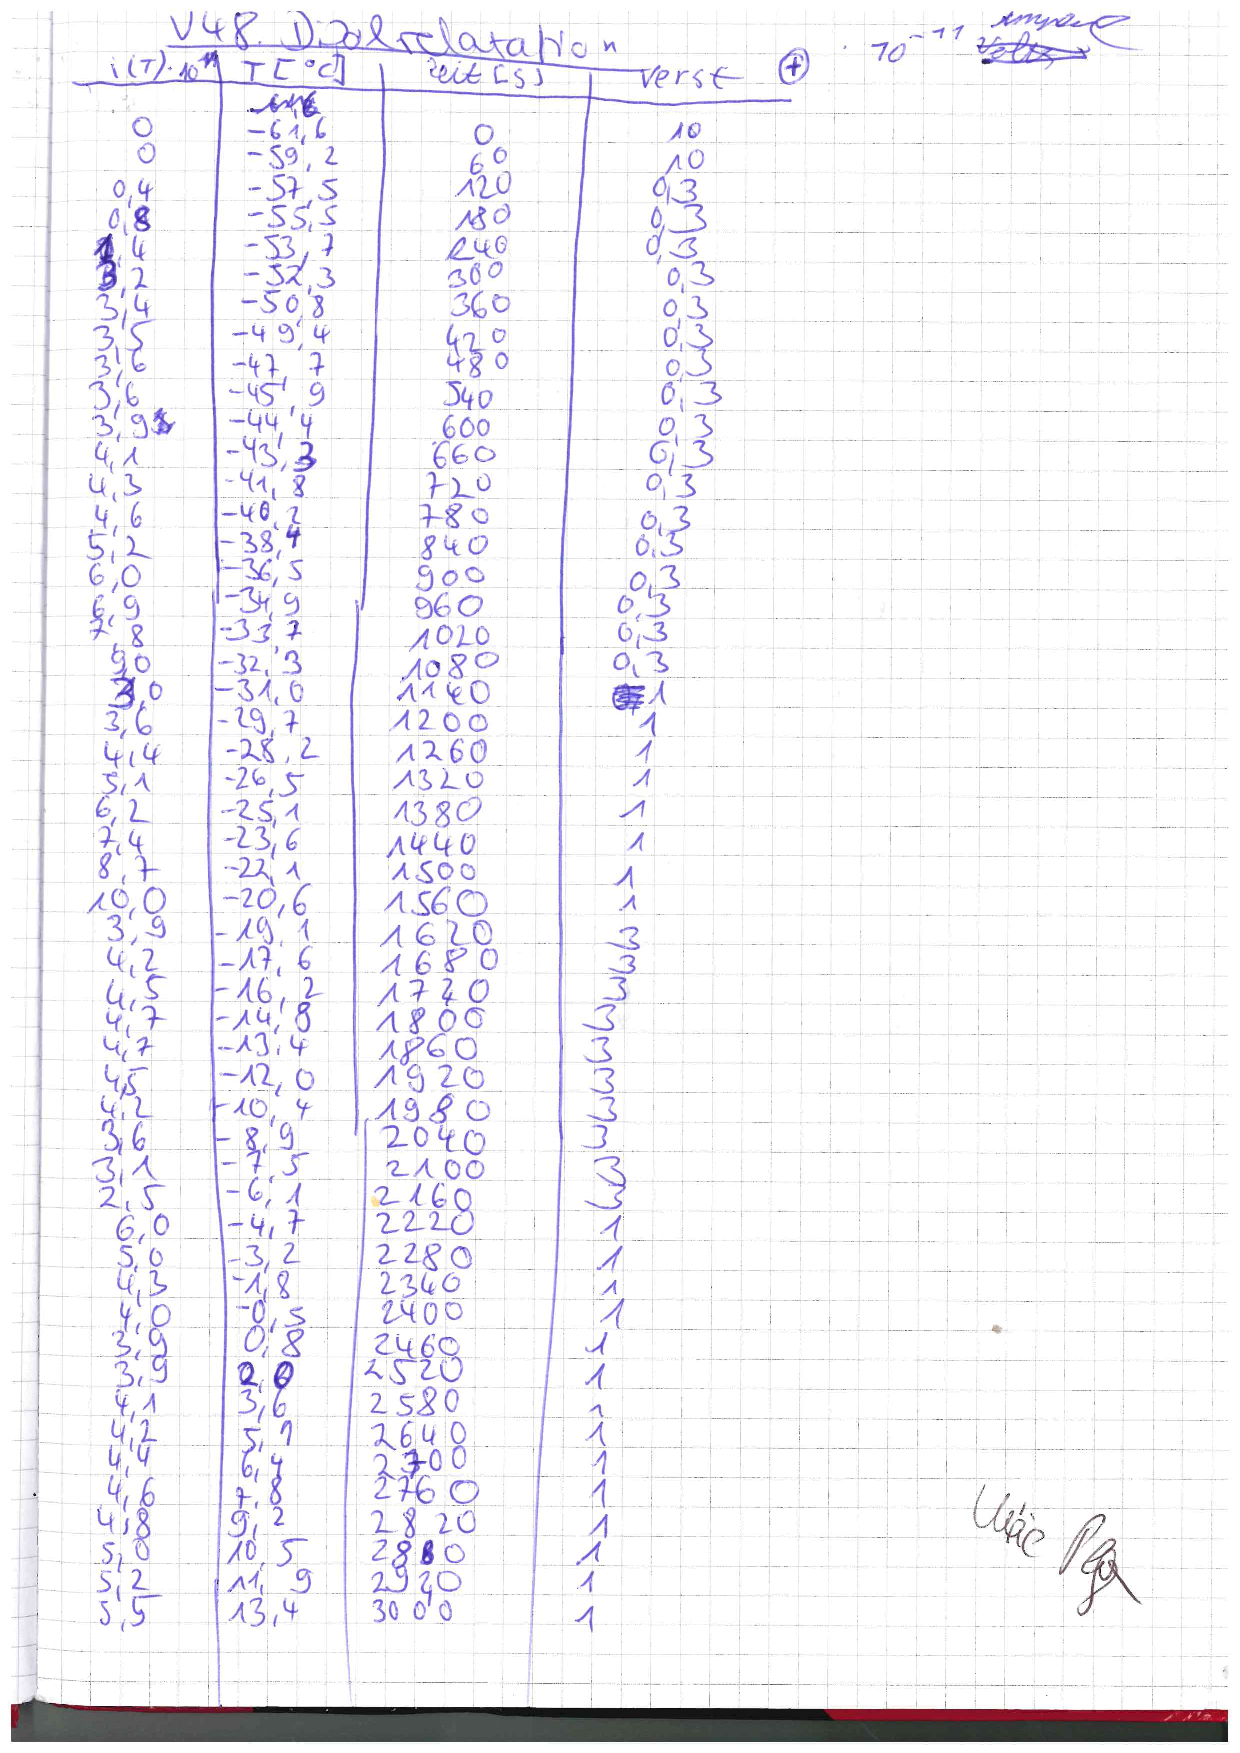
\includegraphics[angle=0, width = \textwidth]{V48-1.pdf}
\end{figure}
\begin{figure}
  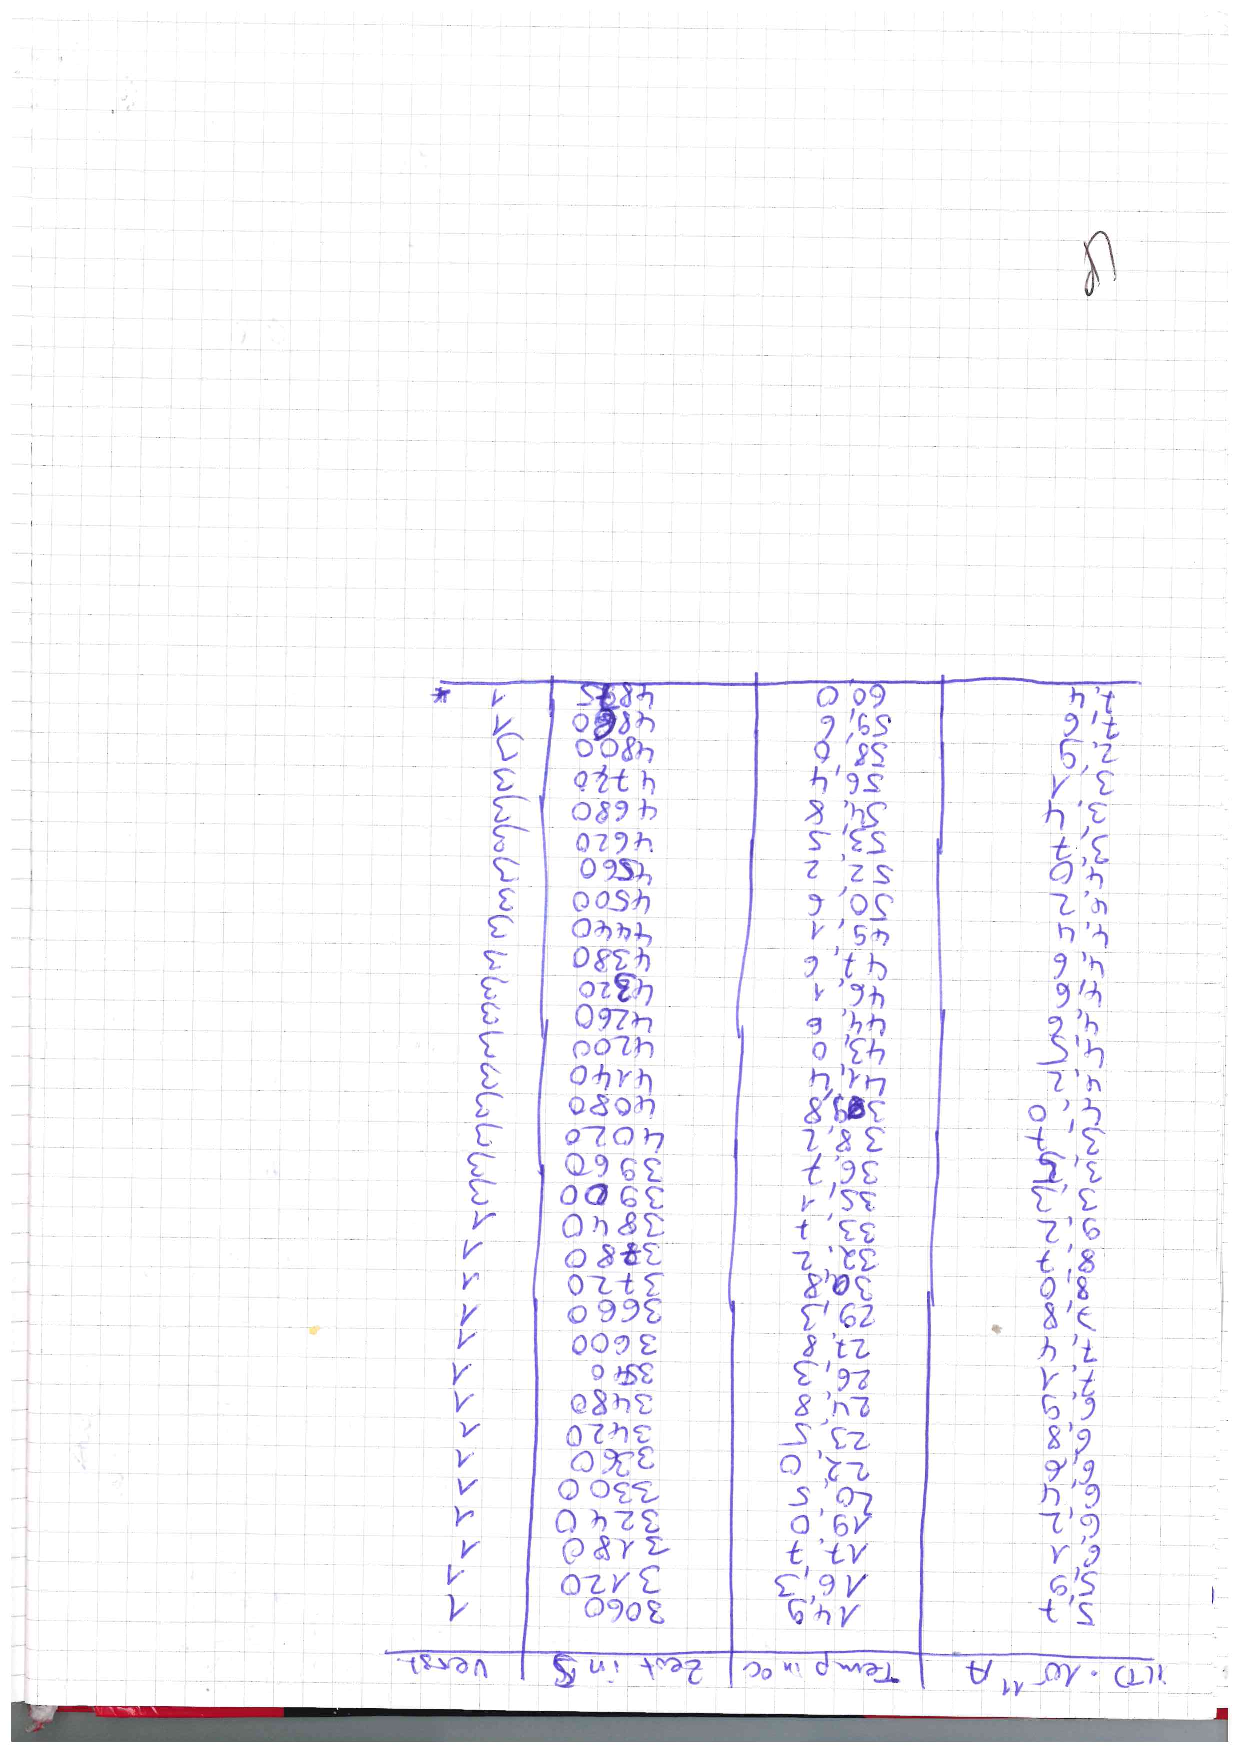
\includegraphics[angle=180, width = \textwidth]{V48-2.pdf}
\end{figure}
\begin{figure}
  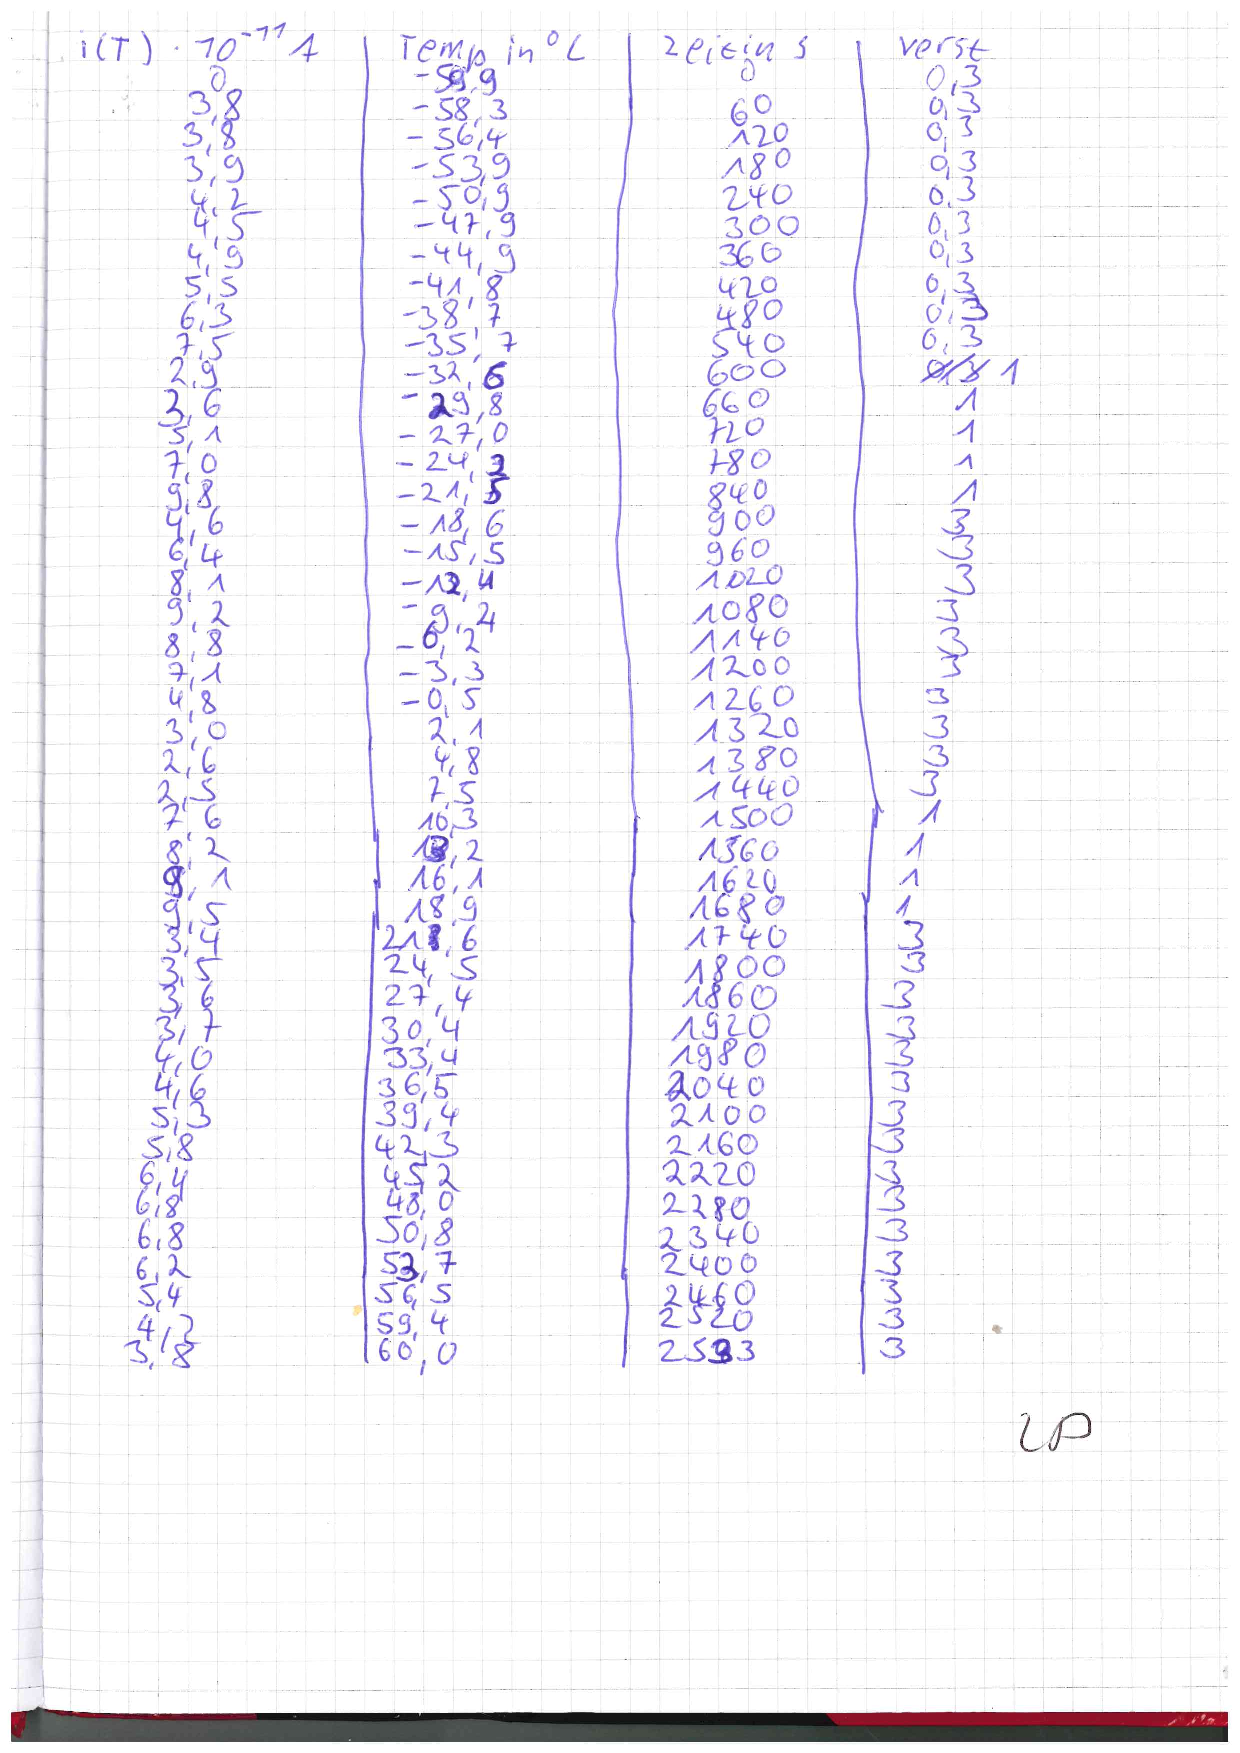
\includegraphics[angle=0, width = \textwidth]{V48-3.pdf}
\end{figure}


\printbibliography

\end{document}
